\documentclass[12pt,a4paper]{report}
\usepackage[utf8]{inputenc}
\usepackage{amsmath}
\usepackage{amsfonts}
\usepackage{amssymb}
\usepackage{makeidx}
\usepackage{graphicx}
\usepackage[left=2cm,right=2cm,top=2cm,bottom=2cm]{geometry}

\begin{document}
\title{\textbf{Sistemas electronicos de interfaz\\Segundo avance de proyecto\\P.I.S.T.O.}}
\author{Alvarez Hernandez Edwin David 18311619\\Arce Montaya Jonathan 18311603\\Briano Garcìa Angel Eraclio 18311625\\Bueno Gòmez Jorge Heriberto 18312259\\Cruz Cervantes Oscar 18311638\\Orozco Nevares Josue Natanael 18311797}
\date{18 de Octubre del 2019}

\begin{figure}
\centering

\includegraphics[width=10cm]{UPCDLZMDG5783-logo.png} 
\end{figure}
\maketitle


\section{Titulo}

P.I.S.T.O. Siguiendo las siglas de nuestro proyecto serian las siguientes:\\
Portador\\
Inteligente\\
Servicial para\\
Tomadores\\
Organizados\\

\subsection{Problematica}
La problematica es que es muy cansado estar preparando las bebidas alcoholicas, ya que te toma mucho tiempo el estar sirviendo los hielos, el alcohol y el refresco, y mas si ya tienes unas copas de mas se complica mas.
Ya que a muchos de nuestros compañeros les ocurre esto fue que decidimos el implementar este mecanismo para evitar el problema planteado.

\section{Cual es el problema a resolver?}
Al realizar la investigacion se determina el problema a resolver, el cual es hacer una distribucion casi perfecta de alcohol en bebidas preparadas (alcoholicas).\\
En la recoleccion de informacion y evidencias notamos que el alcohol se desperdicia en pequenas proporciones que al pasar el tiempo en el evento es una perdida de producto y de dinero.\\
Las razones por la que sucede son diversas, descuidos, vasos con demasiado alcohol y por lo tanto lo dejan de beber o lo tiran, caidas, etc\\El problema por el cual nos vamos a inclinar a resolver sera:\\El suministro adecuado en cada bebida preparada.\\El control y proteccion de las bebidas alcoholicas (para evitar accidentes).\\Un servicio comodo y sencillo de utilizar.\\Rapidez en el servicio.


\section{Objetivo general}
Proponer una propuesta para el mejoramiento de la linea de produccion de produccion de envasado, evaluar sustancialmente la eficiencia de una linea de envasado de bebidas alcoholicas de manera exacta, sin que ello conlleve un coste añadido y en un tiempo reducido.

\section{Objetivos especificos:}
1. Proponer ideas para llevar acabo el proyecto\\2. Diseñar el boceto para ver que necesitamos\\3. Analizar los compotentes que necesitamos.\\4. Comprar los componentes.\\5. Elaborar el proyecto.\\6. Elaborar el programar del plc.\\7. Determinar las pruebas correspondientes.\\8. Analizar si hubo algun error.\\9. Verificar los errores\\10.Dar a conocer el proyecto en la fecha establecida.

\section{Justificacion}
Este proyecto es realizado por la necesidad de facilitar y mejorar procesos de llenado con una mayor precisión, velocidad, y un aumento de la producción, además de reducir los accidentes, perdidas y costos.

\subsection{Delimitacion}
1- El proyecto este programado adecuadamente para su funcionamiento ademas de su correcta construccion.\\
2- Llenar adecuadamente los contenedores de los usuarios que utilicen el P.I.S.T.O. a la medida que el aparato les pueda ofrecer y les otorgue la mayor satisfaccion.\\
3- Economizar en el tema de los recursos al momento de su construccion.
solucion proponemos una maquina automatizada que se encargue de preparar tu bebida alcoholica.

\section{Costos}
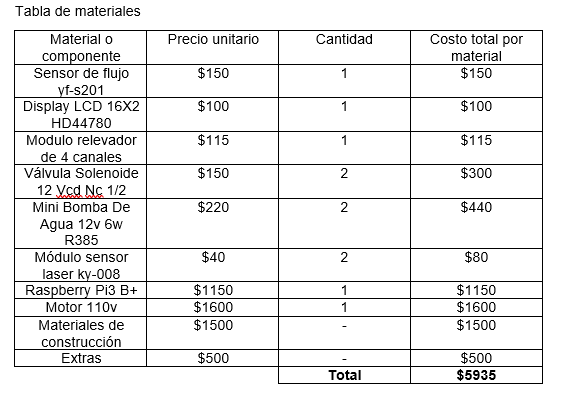
\includegraphics[width=16cm]{Costos.png}

\section{Matriz de roles}
\begin{tabular}{|c|c|}
\hline 
Signo  & Leyenda  \\ 
\hline 
P & Responsabilidad \\ 
\hline 
C & colabora \\ 
\hline 
I & Suministra información a los demás  \\ 
\hline 
NJ & Josué Natanael Orozco Nevares y jonathan Arce Montoya  \\ 
\hline 
EO & Edwin David Álvarez Hernández y Osccar Cruz Cervantes  \\ 
\hline 
BL & Ángel Eraclio Briano García y Lisbeth Martínez Velásquez \\ 
\hline 
\end{tabular} 

\begin{tabular}{|c|c|c|c|c|}
\hline 
Actividades  & NJ & EO & BL & Fecha  \\ 
\hline 
Título del proyecto  & P & I C & C & del 16 al 20 de Sep. 2019 \\ 
\hline 
Planteamiento del problema  & P & I C & C I & del 16 al 20 de Sep. 2019 \\ 
\hline 
Formular el problema  & C & P I & C I & del 16 al 20 de Sep. 2019 \\ 
\hline 
Objetivo general del proyecto  & P & I C & C & del 16 al 20 de Sep. 2019 \\ 
\hline 
Objetivo del proyecto  & C & P I & I C  & del 16 al 20 de Sep. 2019 \\ 
\hline 
Justificación  & C & P I & C & del 16 al 20 de Sep. 2019 \\ 
\hline 
Delimitación & P & I C & I C & del 16 al 20 de Sep. 2019 \\ 
\hline 
Matriz de posibles costos de materiales  & C & I P  & C & del 16 al 20 de Sep. 2019 \\ 
\hline 
Matriz de roles  & C & I & P & del 16 al 20 de Sep. 2019 \\ 
\hline 
Diagrama de Gantt  & C & I & P & del 16 al 20 de Sep. 2019 \\ 
\hline 
Explicación de la aportación de cada materia  & P & I C & C & del 16 al 20 de Sep. 2019 \\ 
\hline 
Desarrollo del proyecto  & P & I & C & del 16 al 20 de Sep. 2019 \\ 
\hline 
Bibliografías  & P C & I & C & del 16 al 20 de Sep. 2019 \\ 
\hline 
Total P & 7 & 4 & 2 & - \\ 
\hline 
Total C & 7 & 5 & 11 & - \\ 
\hline 
Total I & - & 13 & 4 & - \\ 
\hline 
\end{tabular}

\section{Diagrama de Gantt}
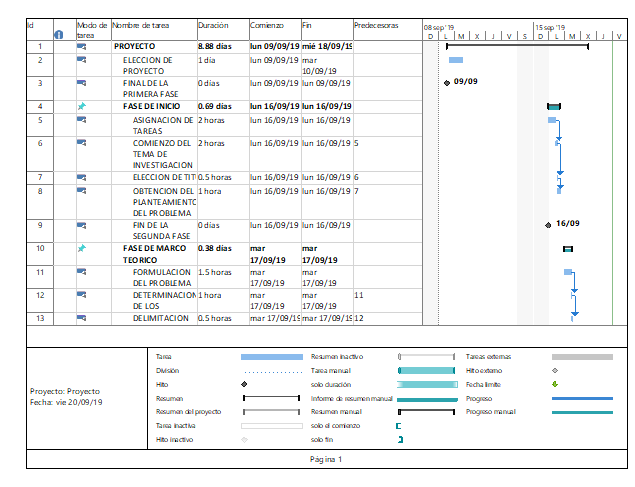
\includegraphics[width=18cm]{Diagrama.png}
\newpage

\section{Materias relacionadas}
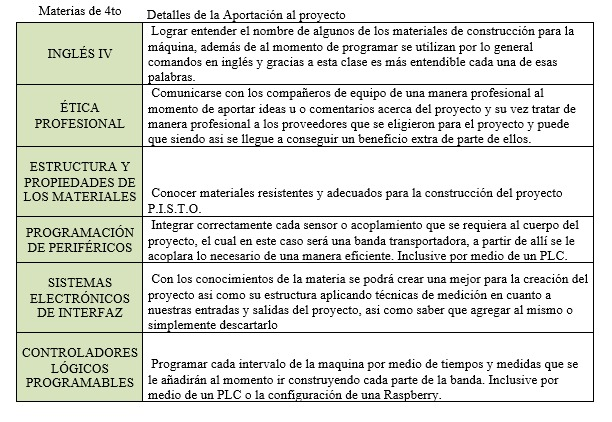
\includegraphics[width=16cm]{materias 2.png}  
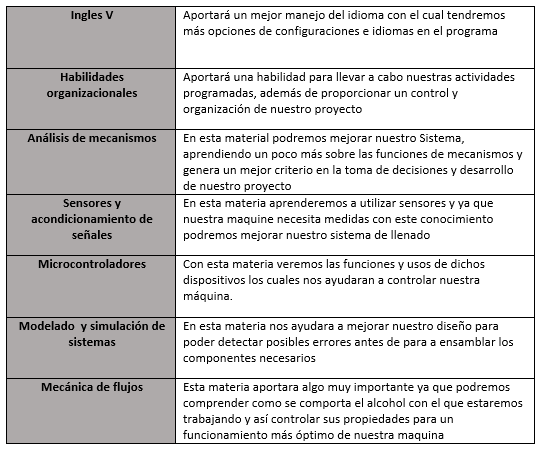
\includegraphics[width=16cm]{Materias.png}
\newpage
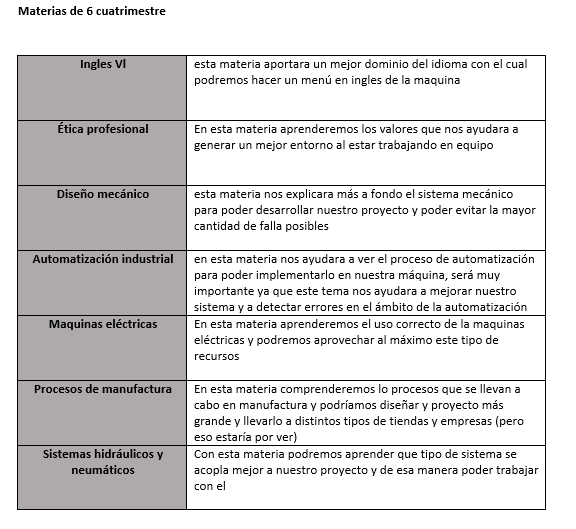
\includegraphics[width=16cm]{Materias1.png} 

\section{Desarrollo}
El desarrollo del proyecto a ido progresando exponencialmente a lo largo de este periodo cuatrimestral, destacando las areas de estudio y apoyo en la cual se a basado nuestro proyecto, refiriendonos a las materias impartidas, por ejemplo:

\subsection{Ingles V}
Gracias a esta materia a sido posible identificar materiales necesarios y componentes de mayor calidad debido a que la mayoria de estos componentes vienen de origen estadounidense.

\subsection{Ètica profesional}
Lograr resolver problemas en el equipo dialogando acerca de los mismo y la organizaciòn adecuada para la construcciòn de este proyecto repartiendo equitativamente los deberes.

\subsection{Estructura y propiedades de los materiales}
Conocimiento adecuado de las sustancias y materiales a necesitar en el proyecto.

\subsection{Programaciòn de perifèricos}
Diseñar el codigo de funcionamiento para el PLC que se le acoplara en el futuro a P.I.S.T.O.

\subsection{Sistemas electrònicos de interfaz}
Diseñar una interfaz adecuada para el usuario que desee interactuar con P.I.S.T.O. Siendo asi sencilla y entendible, sin causar problemas al momento de utilizarlo.

\subsection{Controladores lògicos programables}
Acoplar el PLC a P.I.S.T.O. para su funcionamiento autonomo sin dañar el proposito del mismo.\\

\subsection{Materiales reunidos}
Ademas de lo mencionado, se han adquirido partes para la construcciòn del proyecto, los cuales son:\\
\\

PLC
\begin{figure}[h!]
\centering
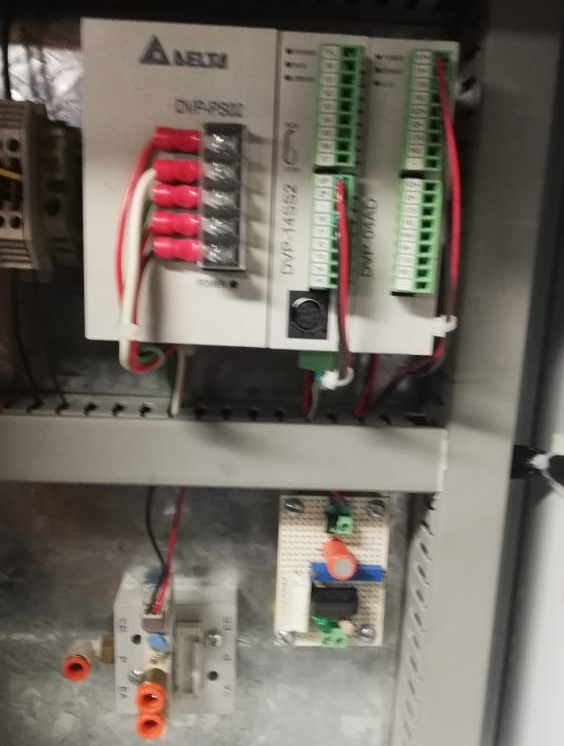
\includegraphics[width=8cm]{PLC.jpg} 
\end{figure}
\newpage

Motor
\begin{figure}[h!]
\centering
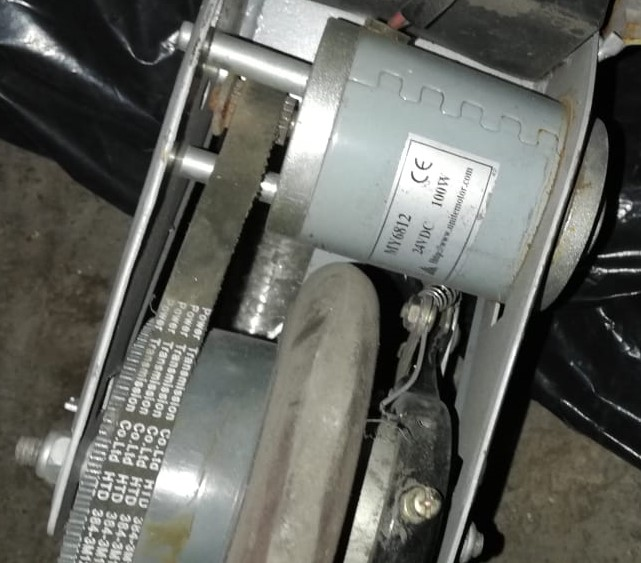
\includegraphics[width=8cm]{Motor.jpg} 
\end{figure}

\cite{manjarr2010}
\bibliographystyle{apalike}
\bibliography{biblio}


\end{document}